
\usepackage{tikz}
\usetikzlibrary{arrows}
\usetikzlibrary{automata,positioning,shapes}

\newcommand{\petersonone}[1][]{
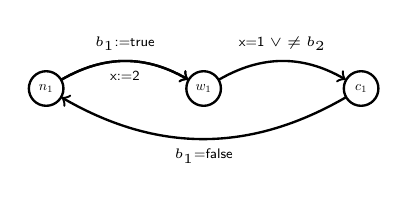
\begin{tikzpicture} [->,auto,node distance=2.0cm,line width=0.3mm]

  \node[state] (1) [scale=0.5]{$n_1$};
  \node[state] (2) [right of=1, scale=0.5] {$w_1$};
  \node[state] (3) [right of=2, scale=0.5] {$c_1$};

  \path[every node/.style={font=\sffamily\tiny}]
    (1) edge [bend left] node [above] {$b_1$:=true} (2)
    (1) edge [bend left] node [below] {x:=2} (2)
    (2) edge [bend left] node [above] {x=1 $\vee$ $\neq$ $b_2$} (3)
    (3) edge [bend left] node [below] {$b_1$=false} (1);

\end{tikzpicture}
}




\newcommand{\petersontwo}[1][]{
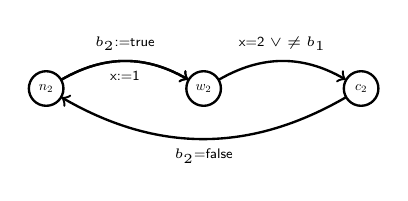
\begin{tikzpicture} [->,auto,node distance=2.0cm,line width=0.3mm]

  \node[state] (1) [scale=0.5]{$n_2$};
  \node[state] (2) [right of=1, scale=0.5] {$w_2$};
  \node[state] (3) [right of=2, scale=0.5] {$c_2$};

  \path[every node/.style={font=\sffamily\tiny}]
    (1) edge [bend left] node [above] {$b_2$:=true} (2)
    (1) edge [bend left] node [below] {x:=1} (2)
    (2) edge [bend left] node [above] {x=2 $\vee$ $\neq$ $b_1$} (3)
    (3) edge [bend left] node [below] {$b_2$=false} (1);

\end{tikzpicture}
}



\newcommand{\petersonboth}[1][]{
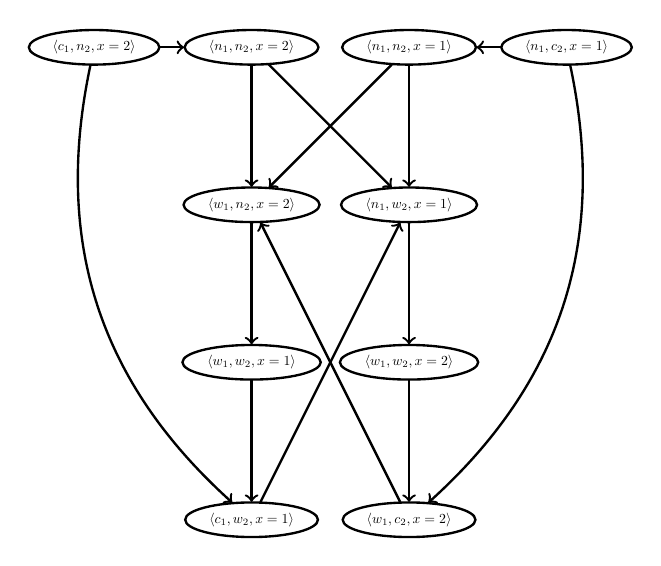
\begin{tikzpicture} [->,auto,node distance=2.0cm,line width=0.3mm]

  \node[state] (1) [ellipse,scale=0.5]{$\langle c_1,n_2,x=2\rangle$};
  \node[state] (2) [ellipse,right of=1, scale=0.5] {$\langle n_1,n_2,x=2\rangle$};
  \node[state] (3) [ellipse,right of=2, scale=0.5] {$\langle n_1,n_2,x=1\rangle$};
  \node[state] (4) [ellipse,right of=3,scale=0.5]{$\langle n_1,c_2, x=1\rangle$};
  \node[state] (5) [ellipse,below of=2, scale=0.5] {$\langle w_1,n_2,x=2\rangle$};
  \node[state] (6) [ellipse,below of=5, scale=0.5] {$\langle w_1,w_2,x=1\rangle$};
  \node[state] (7) [ellipse,below of=6, scale=0.5]{$\langle c_1, w_2,x=1\rangle$};
  \node[state] (8) [ellipse,below of=3, scale=0.5] {$\langle n_1,w_2,x=1\rangle$};
  \node[state] (9) [ellipse,below of=8, scale=0.5] {$\langle w_1,w_2, x=2\rangle$};
  \node[state] (10) [ellipse,below of=9, scale=0.5] {$\langle w_1,c_2,x=2\rangle$};


  \path[every node/.style={font=\sffamily\tiny}]
    (1) edge node [above] {} (2)
        edge [bend right] node [below] {} (7)
    (2) edge  node [below] {} (5)
        edge  node [below] {} (8)
    (3) edge node [above] {} (5)
        edge node [below] {} (8)
    (4) edge node [below] {} (3)
        edge [bend left] node [below] {} (10)
    (5) edge node [below] {} (6)
    (6) edge node [below] {} (7)
    (7) edge node [below] {} (8)
    (8) edge node [below] {} (9)
    (9) edge node [below] {} (10)
    (10) edge node [below] {} (5);



\end{tikzpicture}
}

\newcommand{\burns}[1][]{
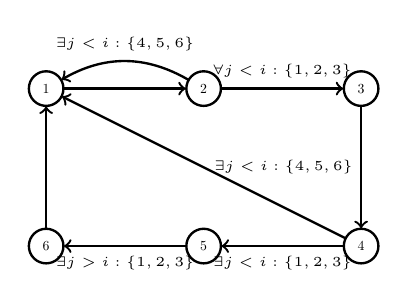
\begin{tikzpicture} [->,auto,node distance=2.0cm,line width=0.3mm]

  \node[state] (1) [scale=0.5]{$1$};
  \node[state] (2) [right of=1, scale=0.5] {$2$};
  \node[state] (3) [right of=2, scale=0.5] {$3$};
  \node[state] (4) [below of=3, scale=0.5] {$4$};
  \node[state] (5) [left of=4, scale=0.5] {$5$};
  \node[state] (6) [left of=5, scale=0.5]{$6$};

  \path[every node/.style={font=\sffamily\tiny}]
    (1) edge node [above] {} (2)
    (2) edge [bend right] node [above] {$\exists j<i: \{4,5,6\}$} (1)
     edge node [above] {$\forall j<i:\{1,2,3\}$} (3)
    (3) edge node [below] {} (4)
    (4) edge node [right] {$\exists j<i: \{4,5,6\}$} (1)
    (4) edge node [below] {$\exists j<i: \{1,2,3\}$} (5)
    (5) edge node [below] {$\exists j>i: \{1,2,3\}$} (6)
    (6) edge node [above] {} (1);
\end{tikzpicture}
}


\newcommand{\abpobserver}[1][]{
\begin{tikzpicture} [->,auto,node distance=3.0cm,line width=0.3mm]

%\begin{tikzpicture}[->,>=stealth',shorten >=1pt,auto,node distance=3cm,
%  thick,main node/.style={circle,fill=blue!20,draw,font=\sffamily\Large\bfseries}]

  \node[scale=0.5, state] (1) {$o_1$};
  \node[scale=0.5,state,accepting] (3) [right of=1] {$o_2$};
  \node[scale=0.5,state] (2) [right of=2] {$o_3$};

  \path[every node/.style={font=\sffamily\tiny}]
    (1) edge [bend left] node [above] {Snd} (2)
        edge node [above] {Rcv} (3)
    (2) edge [bend left] node [below] {Rcv} (1)
        edge node [above] {Snd} (3);
\end{tikzpicture}
}

\newcommand{\abpsender}[1][]{
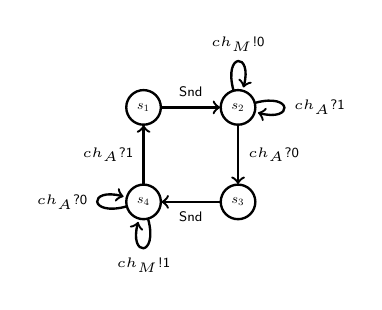
\begin{tikzpicture} [->,auto,node distance=2.4cm,line width=0.3mm]
  \node[scale=0.5,state] (1) {$s_1$};
  \node[scale=0.5,state] (2) [right of=1] {$s_2$};
  \node[scale=0.5,state] (3) [below of=2] {$s_3$};
  \node[scale=0.5,state] (4) [left of=3] {$s_4$};

  \path[every node/.style={font=\sffamily\tiny}]
    (1) edge node [above] {Snd} (2)
    (2) edge node [right] {$ch_A$?0} (3)
        edge [loop right] node {$ch_A$?1} (2)
        edge [loop above] node {$ch_M$!0} (2)
    (3) edge node [below] {Snd} (4)
    (4) edge node [left] {$ch_A$?1} (1)
        edge [loop left] node {$ch_A$?0} (4)
        edge [loop below] node {$ch_M$!1} (4);
\end{tikzpicture}
}

\newcommand{\abpreceiver}[1][]{
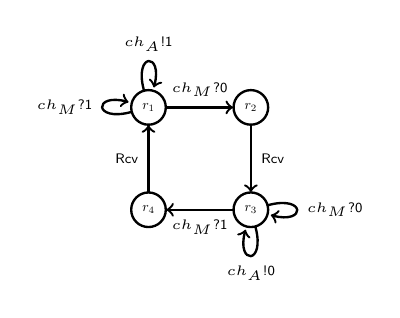
\begin{tikzpicture} [->,auto,node distance=2.6cm,line width=0.3mm]

  \node[scale=0.5,state] (1) {$r_1$};
  \node[scale=0.5,state] (2) [right of=1] {$r_2$};
  \node[scale=0.5,state] (3) [below of=2] {$r_3$};
  \node[scale=0.5,state] (4) [left of=3] {$r_4$};

  \path[every node/.style={font=\sffamily\tiny}]
    (1) edge node [above] {$ch_M$?0} (2)
        edge [loop left] node {$ch_M$?1} (1)
        edge [loop above] node {$ch_A$!1} (1)
    (2) edge node [right] {Rcv} (3)
    (3) edge node [below] {$ch_M$?1} (4)
        edge [loop right] node {$ch_M$?0} (3)
        edge [loop below] node {$ch_A$!0} (3)
    (4) edge node [left] {Rcv} (1);

\end{tikzpicture}
}



\newcommand{\abstraction}[1][]{
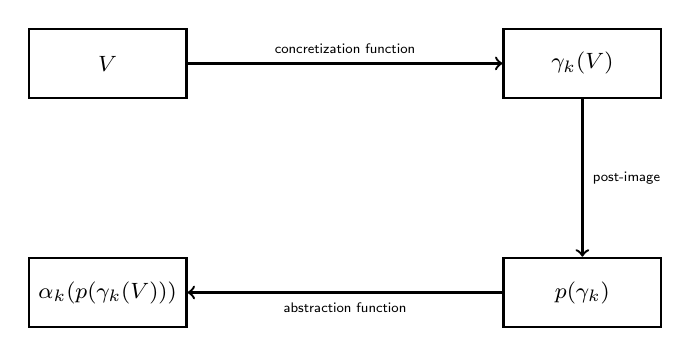
\begin{tikzpicture} [->,auto,node distance=2cm and 4cm,line width=0.3mm, font=\footnotesize]

  \node[state] (1) [rectangle, minimum width=2cm] {$V$};
  \node[state] (2) [rectangle, minimum width=2cm,right=of 1] {$\gamma_k(V)$};
  \node[state] (3) [rectangle, minimum width=2cm,below=of 2] {$p(\gamma_k)$};
  \node[state] (4) [rectangle, minimum width=2cm,left=of 3] {$\alpha_k(p(\gamma_k(V)))$};

  \path[every node/.style={font=\sffamily\tiny}]
    (1) edge node [above] {concretization function} (2)
    (2) edge node [right] {post-image} (3)
    (3) edge node [below] {abstraction function} (4);

\end{tikzpicture}
}
